\documentclass[12pt,t]{beamer}
\usepackage{graphicx}
\usepackage[vlined]{algorithm2e}
\usepackage{times}
\usepackage{calc}
\usepackage{url}
\usepackage{soul}
\usepackage{graphicx}
\usepackage{multirow, hhline}
\usepackage{array, booktabs}
\usepackage{amsmath}
\usepackage{amssymb}
\usepackage{relsize}
\usepackage{multirow}
\usepackage{booktabs}
\usepackage{pagecolor}
\usepackage{lipsum}
\usepackage{capt-of}
\usepackage{booktabs}

\usepackage{graphicx}
\usepackage{multicol}
\usepackage[T1]{fontenc}
\usepackage{ae}
\graphicspath{{fig/}}
\setbeameroption{hide notes}
\setbeamertemplate{note page}[plain]

\usetheme{default}
\beamertemplatenavigationsymbolsempty
\hypersetup{pdfpagemode=UseNone}

\usefonttheme{professionalfonts}
\usefonttheme{serif}
\usepackage{fontspec}
\setmainfont{Karla}
\setbeamerfont{note page}{family*=pplx,size=\footnotesize} % Palatino for notes

\definecolor{foreground}{RGB}{70,70,70}
\definecolor{background}{RGB}{249, 249, 249} %24,24,24
%\definecolor{title}{RGB}{107,174,214} %107,174,214
\definecolor{title}{RGB}{70,70,70}
\definecolor{gray}{RGB}{0,0,0}
\definecolor{subtitle}{RGB}{70,70,70}
\definecolor{hilight}{RGB}{102,255,204}
\definecolor{vhilight}{RGB}{255,111,207}

\setbeamercolor{titlelike}{fg=title}
\setbeamercolor{subtitle}{fg=subtitle}
\setbeamercolor{institute}{fg=gray}
\setbeamercolor{normal text}{fg=foreground,bg=background}


\setbeamercolor{item}{fg=foreground} % color of bullets
\setbeamercolor{subitem}{fg=gray}
\setbeamercolor{itemize/enumerate subbody}{fg=gray}
\setbeamertemplate{itemize subitem}{{\textendash}}
\setbeamerfont{itemize/enumerate subbody}{size=\footnotesize}
\setbeamerfont{itemize/enumerate subitem}{size=\footnotesize}

\setbeamercolor{block title}{fg=white,bg=gray!70}
\setbeamercolor{block body}{fg=black,bg=gray!10}
\setbeamercolor{block title alerted}{fg=red,bg=gray!40}
\setbeamercolor{block title example}{fg=black,bg=green!20}
\setbeamercolor{block body example}{fg=black,bg=green!5}
\setbeamerfont{block title}{series=\bfseries}

\hypersetup{colorlinks,linkcolor=foreground,urlcolor=foreground}


\setbeamertemplate{footline}{%
    \raisebox{5pt}{\makebox[\paperwidth]{\hfill\makebox[20pt]{\color{gray}
          \scriptsize\insertframenumber}}}\hspace*{5pt}}

\addtobeamertemplate{note page}{\setlength{\parskip}{12pt}}


\newcommand{\bi}{\begin{itemize}}
\newcommand{\ei}{\end{itemize}}
\newcommand{\ig}{\includegraphics}
\newcommand{\subt}[1]{{\footnotesize \color{subtitle} {#1}}}

\let\emph\relax % there's no \RedeclareTextFontCommand
\DeclareTextFontCommand{\emph}{\bfseries\em}


\setbeamertemplate{frametitle}
{\vskip4pt
  \leavevmode
%\hbox{%
\begin{beamercolorbox}[wd=\paperwidth,ht=2ex,dp=0ex]{frametitle}%
\underline{\makebox[\paperwidth][l]{\hspace*{10pt}
\large {{\insertframetitle}}}}
\end{beamercolorbox}
%  }%
}

%\setbeamercolor{frametitle}{fg=yellow,bg=red}

\begin{document}

\AtBeginSection[]{
  \begin{frame}
  \vfill
  \centering
  \begin{beamercolorbox}[sep=8pt,center,shadow=true,rounded=true]{title}
    \underline{\makebox[0.6\paperwidth][l]{
\large {{\insertsectionhead}}}}
  \end{beamercolorbox}
  \vfill
  \end{frame}
}

\title{\large{Lecture \#15: Regression Trees \& Random Forests}}
\subtitle{CS 109A, STAT 121A, AC 209A: Data Science}
\author{Pavlos Protopapas \and Kevin Rader}
%\institute{Harvard University}
\date{}
\titlegraphic{
   
\includegraphics[height=2cm]{iacs}
\includegraphics[height=2cm]{hogwarts}
}
{
\setbeamertemplate{footline}{} % no page number here
\frame{
  \titlepage
  
}
}


\begin{frame}{Lecture Outline}
\tableofcontents
\end{frame}

%%%%%%%%%%%%%%%%%%%%%%%%%%%%%%%%%%%%%%%%%%%%%%%%%%%%%%%%%%%%%%%%%%%%%%%%%%%%%%
\section{Review}

%%%%%%%%%%%%%%
\begin{frame}{Decision Trees} 
\vskip-0.4cm
\small
A \emph{decision tree model} is an interpretable model in which the final output is based on a series of comparisons of the values of predictors against threshold values. 
\vskip0.2cm
Graphically, decision trees can be represented by a flow chart. 
\vskip0.2cm
Geometrically, the model partitions the feature space wherein each region is assigned a response variable value based on the training points contained in the region.
\vskip0.4cm
\begin{center}
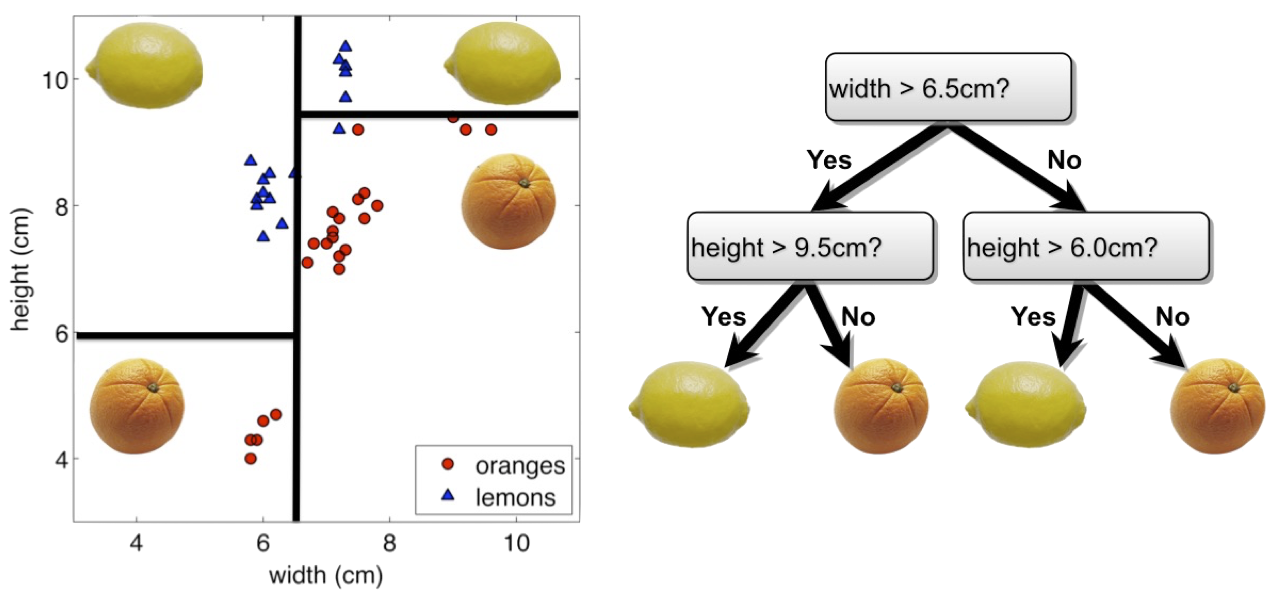
\includegraphics[width=90mm]{lecture14_g8}
\end{center}
\end{frame}

%%%%%%%%%%%%%%
\begin{frame}{Learning Algorithm} 
\vskip-0.4cm
To learn a decision tree model, we take a greedy approach:
\vskip0.2cm
\begin{enumerate}
\item Start with an empty decision tree (undivided feature space)
\item Choose the `optimal' predictor on which to split and choose the `optimal' threshold value for splitting by applying a \emph{splitting criterion}
\item Recurse on on each new node until \emph{stopping condition} is met
\end{enumerate}
\vskip0.2cm
For classification, we label each region in the model with the label of the class to which the plurality of the points within the region belong.
\end{frame}

%%%%%%%%%%%%%%%%%%%%%%%%%%%%%%%%%%%%%%%%%%%%%%%%%%%%%%%%%%%%%%%%%%%%%%%%%%%%%%
\section{Decision Trees for Regression}

%%%%%%%%%%%%%%
\begin{frame}{Adaptations for Regression} 
\footnotesize
\vskip-0.4cm
With just two modifications, we can use a decision tree model for regression:
\vskip0.2cm
\begin{itemize}
\item The three splitting criteria we've examined each promoted splits that were pure - new regions increasingly specialized in a single class. 
\vskip0.2cm
For classification, purity of the regions is a good indicator the performance of the model.
\vskip0.2cm
For regression, we want to select a splitting criterion that promotes splits that improves the predictive accuracy of the model as measured by, say, the MSE.
\vskip0.2cm
\item For regression with output in $\mathbb{R}$, we want to label each region in the model with a real number - typically the average of the output values of the training points contained in the region.
\end{itemize}
\end{frame}

%%%%%%%%%%%%%%
\begin{frame}{Learning Regression Trees} 
\vskip-0.4cm
\footnotesize
The learning algorithms for decision trees in regression tasks is:
\vskip0.2cm
\begin{enumerate}
\item Start with an empty decision tree (undivided feature space)
\item Choose a predictor $j$ on which to split and choose a threshold value $t_j$ for splitting such that the weighted average MSE of the new regions as smallest possible:
\[
\mathrm{argmin}_{j, t_j}  \frac{N_1}{N} \mathrm{MSE}(R_1) +  \frac{N_2}{N} \mathrm{MSE}(R_2) 
\]
or equivalently,
\[
\mathrm{argmin}_{j, t_j}  \frac{N_1}{N} \mathrm{Var}[y | x\in R_1] + \frac{N_2}{N} \mathrm{Var}[y |  x\in R_2]
\]
where $N_i$ is the number of training points in $R_i$ and $N$ is the number of points in $R$.
\item Recurse on on each new node until \emph{stopping condition} is met
\end{enumerate}
\end{frame}

%%%%%%%%%%%%%%
\begin{frame}{Stopping Conditions} 
\vskip0.2cm
Most of the stopping conditions, like maximum depth or minimum number of points in region, we saw last time can still be applied. 
\vskip0.2cm
In the place of purity gain, we can instead compute accuracy gain for splitting a region $R$
\[
\text{Gain}(R) = \Delta(R) = MSE(R) - \frac{N_1}{N} MSE(R_1) -  \frac{N_2}{N} MSE(R_2)
\]
and stop the tree when the gain is less than some pre-defined threshold.
\end{frame}

%%%%%%%%%%%%%%
\begin{frame}{Expressiveness of Decision Trees} 
\only<1>{
\vskip-0.2cm
\small
We've seen that classification trees approximate boundaries in the feature space that separate classes.
\vskip0.2cm
Regression trees, on the other hand, define \emph{simple functions} or step functions, functions that are defined on partitions of the feature space and are constant over each part.
\vskip0.2cm
\begin{center}
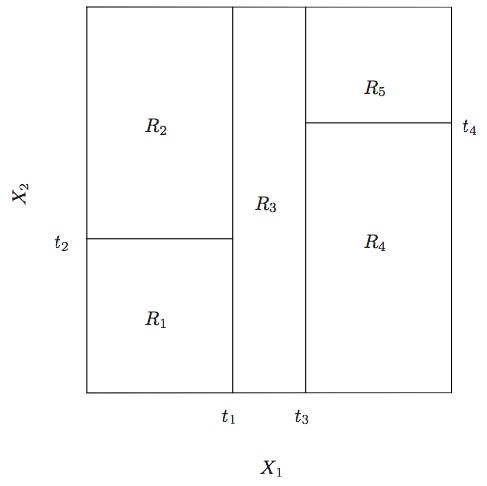
\includegraphics[height=35mm]{lecture15_g1}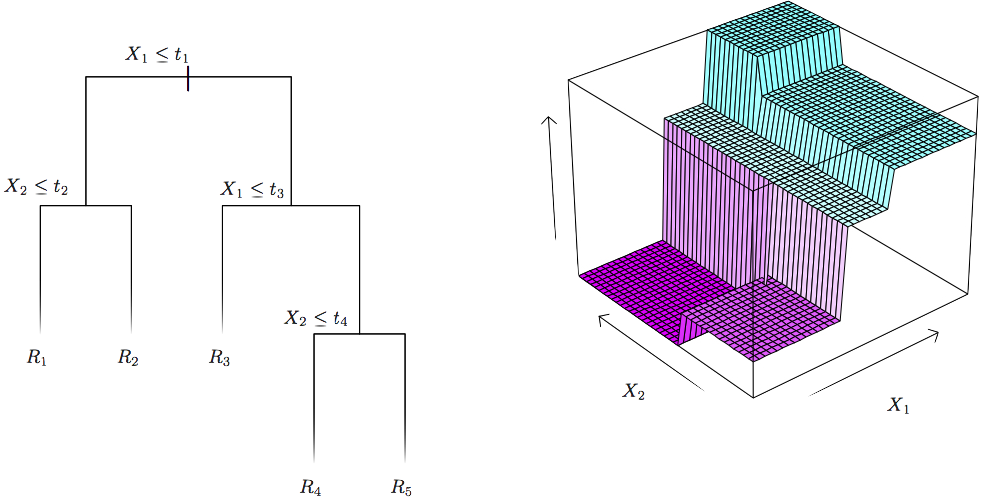
\includegraphics[height=35mm]{lecture15_g2}
\end{center}
}
\only<2>{
For a fine enough partition of the feature space, these functions can approximate complex non-linear functions. 
\begin{center}
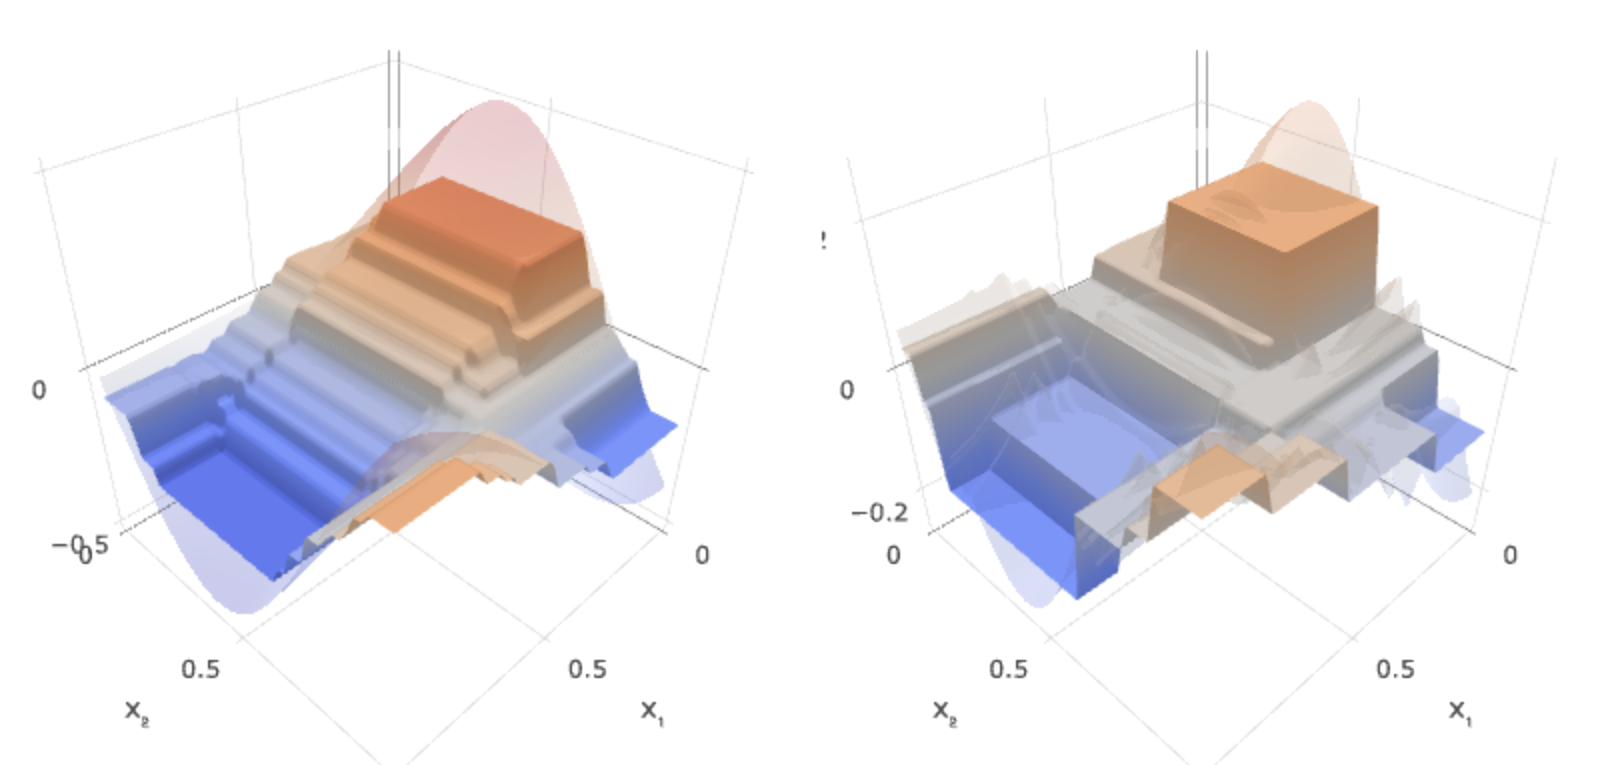
\includegraphics[width=100mm]{lecture15_g3}
\end{center}
}
\end{frame}

%%%%%%%%%%%%%%%%%%%%%%%%%%%%%%%%%%%%%%%%%%%%%%%%%%%%%%%%%%%%%%%%%%%%%%%%%%%%%%
\section{Bagging}

%%%%%%%%%%%%%%
\begin{frame}{Limitations of Decision Tree Models} 
Decision trees models are highly interpretable and fast to train, using our greedy learning algorithm.
\vskip0.2cm
However, in order to capture a complex decision boundary (or to approximate a complex function), we need to use a large tree (since each time we can only make axis aligned splits). 
\vskip0.2cm
We've seen that large trees have high variance and are prone to overfitting.
\vskip0.2cm
For these reasons, in practice, decision tree models often underperforms when compared with other classification or regression methods.
\end{frame}

%%%%%%%%%%%%%%
\begin{frame}{Bagging} 
\only<1>{
\vskip-0.4cm
\small
One way to adjust for the high variance of the output of an experiment is to perform the experiment multiple times and then average the results. 
\vskip0.2cm
The same idea can be applied to high variance models:
\begin{enumerate}
\item \textbf{(Bootstrap)} we generate multiple samples of training data, via bootstrapping. We train a full decision tree on each sample of data.
\item \textbf{(Aggregate)} for a given input, we output the averaged outputs of all the models for that input. 
\vskip0.2cm
For classification, we return the class that is outputted by the plurality of the models.
\end{enumerate}
This method is called \emph{Bagging} (Breiman, 1996), short for, of course, Bootstrap Aggregating. 
}

\only<2>{
Note that bagging enjoys the benefits of
\vskip0.2cm
\begin{enumerate}
\item High expressiveness - by using full trees each model is able to approximate complex  functions and decision boundaries.
\item Low variance - averaging the prediction of all the models reduces the variance in the final prediction, assuming that we choose a sufficiently large number of trees.
\end{enumerate}
}

\only<3>{
\vskip-0.4cm
\begin{center}
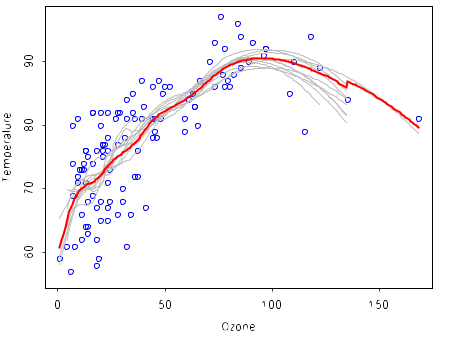
\includegraphics[width=90mm]{lecture15_g4}
\end{center}
}

\only<4>{
However, the major drawback of bagging (and other \emph{ensemble methods} that we will study) is that the averaged model is no longer easily interpretable - i.e. one can no longer trace the `logic' of an output through a series of decisions based on predictor values!
}

\only<5>{
\vskip-0.4cm
\begin{center}
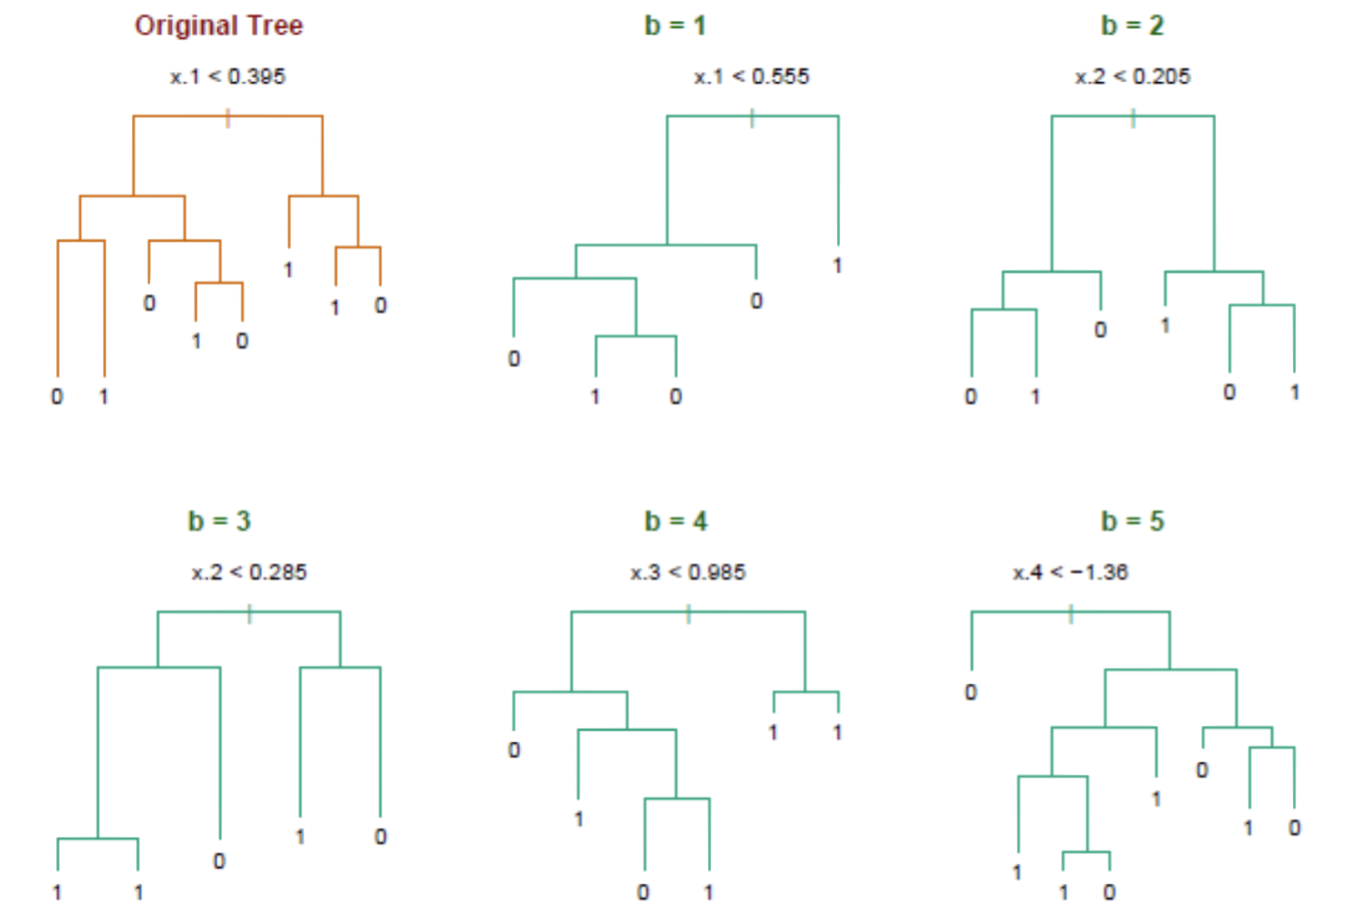
\includegraphics[width=100mm]{lecture15_g5}
\end{center}
}
\end{frame}

%%%%%%%%%%%%%%
\begin{frame}{Out-of-Bag Error} 
\vskip-0.4cm
\footnotesize
Bagging is an example of an \emph{ensemble method}, a method of building a single model by training and aggregating multiple models.
\vskip0.2cm
With ensemble methods, we get a new metric for assessing the predictive performance of the model, the \emph{out-of-bag error}.
\vskip0.2cm
Given a training set and an ensemble of modeled each trained on a bootstrap sample, we compute the \emph{out-of-bag error} of the averaged model by
\vskip0.2cm
\begin{enumerate}
\item for each point in the training set, we average the predicted output for this point over the models whose bootstrap training set excludes this point. 
\vskip0.2cm
We compute the the error or squared error of this averaged prediction. Call this the point-wise out-of-bag error.
\item we average the point-wise out-of-bag error over the full training set.
\end{enumerate}
\end{frame}

%%%%%%%%%%%%%%%%%%%%%%%%%%%%%%%%%%%%%%%%%%%%%%%%%%%%%%%%%%%%%%%%%%%%%%%%%%%%%%
\section{Random Forests}

%%%%%%%%%%%%%%
\begin{frame}{Improving on Bagging} 
\only<1>{
In practice, the ensembles of trees in Bagging tend to be highly correlated. 
\vskip0.2cm
Suppose we have an extremely strong predictor, $x_j$, in the training set amongst moderate predictors. Then the greedy learning algorithm ensures that most of the models in the ensemble will choose to split on $x_j$ in early iterations.
\vskip0.2cm
That is, each tree in the ensemble is identically distributed, with the expected output of the averaged model the same as the expected output of any one of the trees.
}

\only<2>{
Recall, for $B$ number of identically but not independently distributed variables with pairwise correlation $\rho$ and variance $\sigma^2$, the variance of their mean is
\[
\rho \sigma^2 + \frac{1- \rho}{B}\sigma^2.
\]
As we increase $B$, the second term vanishes but the first term remains. 
\vskip0.2cm
Consequently, variance reduction in bagging is limited by the fact that we are averaging over highly correlated trees.
}
\end{frame}

%%%%%%%%%%%%%%
\begin{frame}{Random Forests} 
\emph{Random Forest} is a modified form of bagging that creates ensembles of independent decision trees. 
\vskip0.2cm
To de-correlate the trees, we:
\begin{enumerate}
\item train each tree on a separate bootstrap sample of the full training set (same as in bagging)
\vskip0.2cm
\item for each tree, at each split, we \emph{randomly} select a set of $J'$ predictors from the full set of predictors. 
\vskip0.2cm
From amongst the $J'$ predictors, we select the optimal predictor and the optimal corresponding threshold for the split. 
\end{enumerate}
\end{frame}

%%%%%%%%%%%%%%
\begin{frame}{Tuning Random Forests} 
\only<1>{
Random forest models have multiple hyper-parameters to tune:
\vskip0.2cm
\begin{enumerate}
\item the number of predictors to randomly select at each split
\item the total number of trees in the ensemble
\item the minimum leaf node size
\end{enumerate}
\vskip0.2cm
In theory, each tree in the random forest is full, but in practice this can be computationally expensive (and added redundancies in the model), thus, imposing a minimum node size is not unusual.
}

\only<2>{
There are standard (default) values for each of random forest hyper-parameters recommended by long time practitioners, but generally these parameters should be tuned through cross validation (making them data and problem dependent).
\vskip0.2cm
Using out-of-bag errors, training and cross validation can be done in a single sequence - we cease training once the out-of-bag error stabilizes
}
\end{frame}

%%%%%%%%%%%%%%
\begin{frame}{Example} 
[compare RF, Bagging and Tree]x

[test for variable importance]
\end{frame}

%%%%%%%%%%%%%%
\begin{frame}{Final Thoughts on Random Forests} 
\vskip-0.4cm
\small
\begin{itemize}
\only<1>{
\item When the number of predictors is large, but the number of relevant predictors is small, random forests can perform poorly.
\vskip0.2cm
In each split, the chances of selected a relevant predictor will be low and hence most trees in the ensemble will be weak models.
\vskip0.2cm
}
\only<2>{
\item Increasing the number of trees in the ensemble generally does not increase the risk of overfitting. 
\vskip0.2cm
Again, by decomposing the generalization error in terms of bias and variance, we see that increasing the number of trees produces a model that is at least as robust as a single tree.
\vskip0.2cm
However, if the number of trees is too large, then the trees in the ensemble may become more correlated, increase the variance.
}
\end{itemize}
\end{frame}

\end{document}
